
\chapter{Detection of man-made structures with satellites} 

\label{Chapter5}

%----------------------------------------------------------------------------------------

In this chapter we discuss the results obtained in this thesis. We first evaluate for different resolutions the performance of the Deep Learning pipeline that was described in the previous chapter. Subsequently we discuss several examples of correctly and wrongly classified images. In the last part of the chapter, we estimate the cost associated with providing earth observation data involving satellites.

\section{Man-made structures detection at different scale}

Having indicated in the last chapter that the developed transfer learning approach achieves remarkable accuracies, we now turn to a more detailed and explicit study. We evaluate how the trained model, that is based on a pre-trained ResNet as feature extractor for aerial images, allows to properly discriminate the existence of human impact for different resolutions, different datasets, different categories, different ResNet terminations, and different cross-validation folds. The results for all these experiments have been aggregated and are shown in Fig.~\ref{fig:acc_res_03m_1m} as well as summarized in tables \ref{tab:Results_03m_100n}-\ref{tab:Results_1m_200n} in the appendix. 

The highest accuracy, 95.7\%, is achieved at a resolution of 0.6m for the dataset with 0.3m base resolution and a fully connected layer with 200 neurons. The lowest accuracy, 78.1\%, is obtained at 14m resolution for the architecture with the fully connected layer with 100 neurons. As expected, the accuracy decreases roughly linearly as the resolution becomes worse. However, between 0.3m and 8m the accuracies are consistently above 88\%, and only drop below 85\% at resolution values higher than 8m. At these high values for the resolution the model is not able anymore to detect subtle elements of man-made structures, which will be discussed in more detail in section \ref{seq:selected_images}.

We further note that the accuracy on the base resolution (0.3m and 1m) is always slightly worse than the accuracy at the next resolution. We suspect that this anomaly is related to the fact that the input image size is quite large ($512\times512$), which makes the dense layer more complex to train. Indeed, Figs.~\ref{fig:conv_plots_03m} and \ref{fig:conv_plots_1m} in chapter \ref{Chapter4} suggest that the models struggle to be optimized. More sample images would be required in order to compensate for the complexity and hence to achieve a higher accuracy.

\begin{figure}[h!]
	\centering
	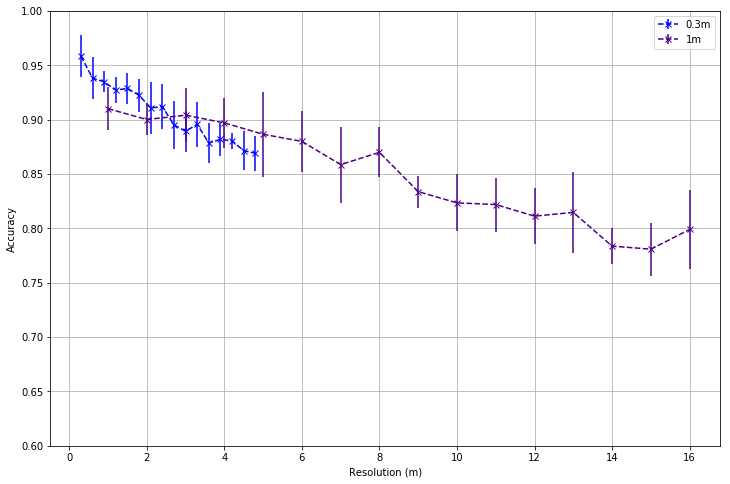
\includegraphics[width=0.8\textwidth]{Figures/results/acc_res_03m_1m.png}
	\captionsetup{width=1\linewidth}
	\caption{\textbf{Accuracy at each resolution for all datasets and architectures.} The blue (purple) lines correspond to the 0.3m (1m) dataset and lighter (darker) color belongs to a 100 (200) neurons architecture. The 0.3m (1m) dataset was trained and evaluated on a total of $\sim$2000 ($\sim$1300) images. Note that, however the base resolution of the 0.3m dataset was trained and evaluated with only 1500 images, because Colab's memory requirements did not allow to process more images with size $512\times512$. The vertical lines represent the variability (standard deviation) for the different folds of the 8-fold cross-validation.}
	\label{fig:acc_res_03m_1m}
\end{figure}

The architecture with the fully connected layer with 200 neurons performs slightly better than the one with 100 neurons, but accuracy improvements are generally in the range of 1\% - 2\%. Hence, we will focus on the 200 neurons architecture from now on. Another important observation is that at the region where the resolutions overlap between the two datasets also the accuracies agree i.e. they are within the error bars. This indicates that both datasets are comparable and can be considered together.
Note that the error bars of the 1m dataset ($\sim$1300 images) are about twice as large as the error bars for the 0.3m dataset ($\sim$2000 images). The larger variation for the 1m dataset is attributed to the different sizes of the datasets, and hence significantly different number of out-of-fold samples.

\section{Man-made structures detection for different categories}

Let us consider how the accuracies behave for each of the USGS land use categories. As discussed in section \ref{usgs_data}, these categories are rough approximations of the kind of terrain and human impact, but we can not assure with absolute certainty that every image is assigned to the correct category. Fig.~\ref{fig:acc_by_cat_03m} shows a comparison of the accuracy of each category with respect to the aggregated accuracy. For the 0.3m dataset (and 200 neurons model) we observe that there are substantial differences between categories. 

\begin{figure}[h!]
	\centering
	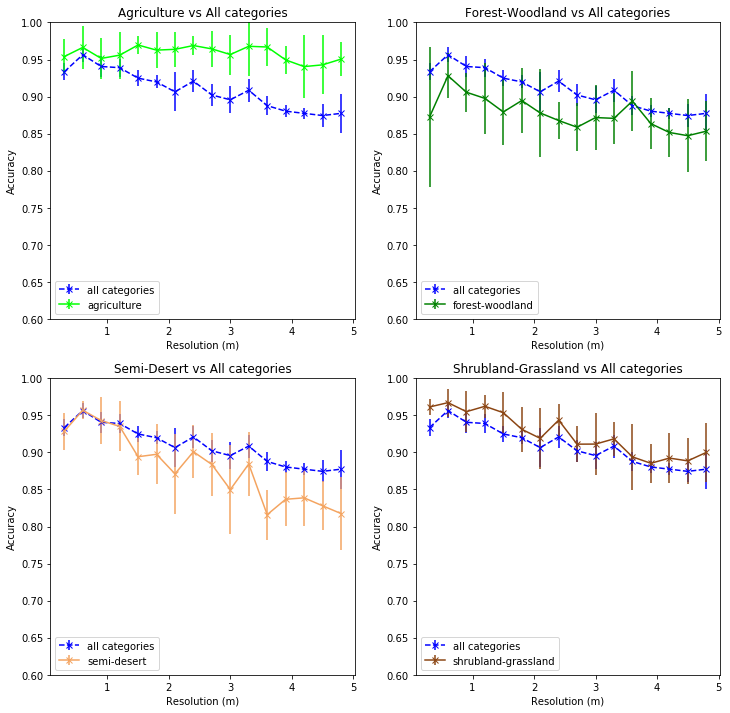
\includegraphics[width=0.9\textwidth]{Figures/results/acc_res_by_category_03m.png}
	\captionsetup{width=1\linewidth}
	\caption{\textbf{Comparison of accuracies between each category and all categories aggregated.} Here the model is trained over all categories, on the 0.3m dataset, and tested on each category separately.}
	\label{fig:acc_by_cat_03m}
\end{figure}

These plots have been obtained once the model was trained for all the categories. Then, the accuracy on the validation set was computed for each individual category and over all images in the set. The validation set in each iteration of the cross-validation was small, consisting of few hundred images, and a homogeneous representation of the categories was not imposed (validation samples were picked randomly, only preserving proportion between man-made vs. natural structures), which explains the large variability for each experiment (large error bars).

Although the category is not taken into account when training, we can see that the models are capable of detecting agriculture-related human impact with an accuracy consistently above 95\%, without being affected by the drop in resolution. This is not surprising since this category contains only images with man-made structures, and therefore the algorithm might indeed have learned image textures instead of features related to human impact.
The shrubland-grassland category has about 2\% higher accuracy than all categories, while the resolution dependence is similar. The forest-woodland category is  about 4\% worse than the overall also showing a similar resolution dependence. Finally, the semi-desert category starts off at the same accuracy as all categories at high resolutions but drops siginificantly faster down to about 82\% (all categories ~88\%). Overall we conclude, that each of the three non-agriculture categories encode slightly different image features, and therefore the algorithm behaves slightly different.

Similar results are obtained on the 1m dataset, which are shown in Fig.~\ref{fig:acc_by_cat_1m}. The models are able to achieve a remarkable accuracy when detecting agriculture-related human impact (consistently above $95\%$), and the three non-agriculture categories behave similar to the aggregated view. However, we note a drop of accuracy at 8m resolution by about 5\% across all non-agriculture categories, which is an indicator that many man-made structures in the dataset have a characteristic size of  about 8m.

\begin{figure}[H]
	\centering
	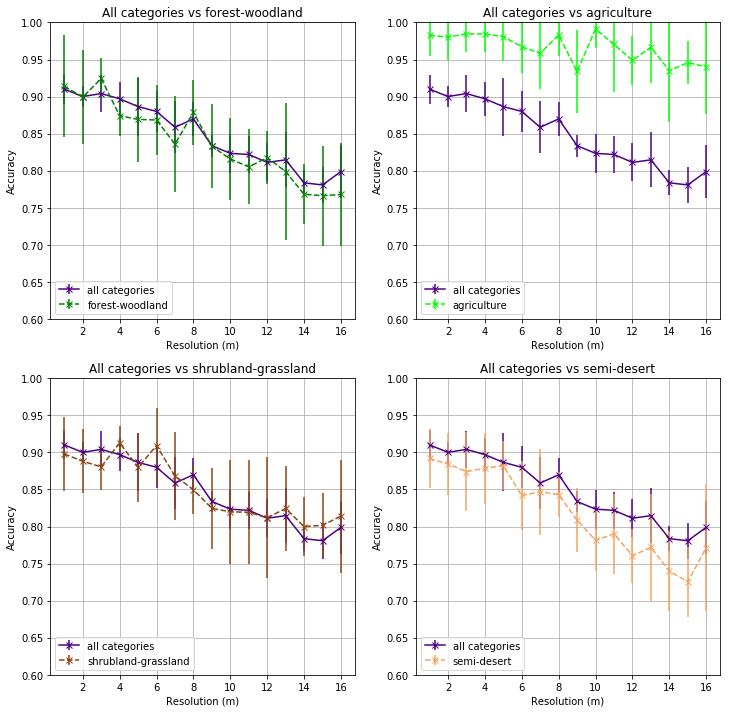
\includegraphics[width=0.9\textwidth]{Figures/results/acc_res_by_category_1m.png}
	\captionsetup{width=1\linewidth}
	\caption{\textbf{Comparison of accuracies between each category and all categories aggregated.} Here the model is trained over all categories, on the 1m dataset, and tested on each category separately (in the case of a single category).}
	\label{fig:acc_by_cat_1m}
\end{figure}


\subsection{Performance on selected images}
\label{seq:selected_images}
In this subsection we will illustrate the algorithm behaviour by considering concrete examples of correctly and wrongly classified images. In Figs.~\ref{fig:dataset03m_res03_correct} and \ref{fig:dataset03m_res03_wrong} we show examples for the 0.3m dataset at base resolution (for one of the cross-validation folds), respectively.
The first set of samples (Fig.~\ref{fig:dataset03m_res03_correct}) shows that the model accurately detects clear human impact related to agriculture (2nd picture in the second row) and paths. On the other hand, the second set (Fig.~\ref{fig:dataset03m_res03_wrong}) indicates that it might fail to detect it when the impact is subtle, covering a small region of the image, or when it can even be confused with natural structures (or vice versa). Note that in this subsection we refere to images with clear human impact as images with label 1 (in contrast to chapter~\ref{Chapter2} where they were defined as label 2).

\begin{figure}[H]
	\centering
	\captionsetup{width=1\linewidth}
	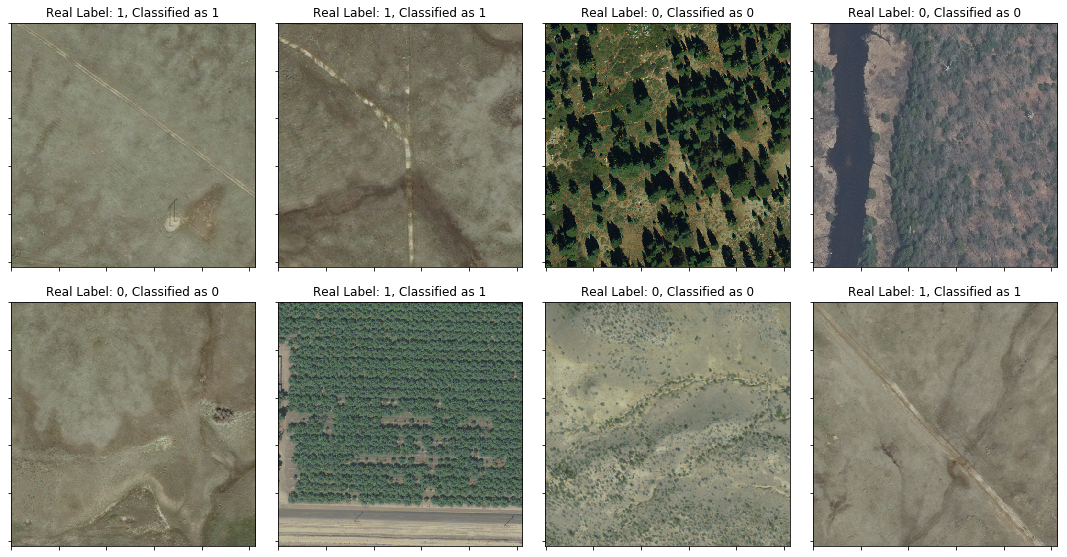
\includegraphics[width=1\textwidth]{Figures/results/class_dataset03m_res03_correct.png}
	\caption{\textbf{Examples of correctly classified images at base resolution of 0.3m dataset.} The title of each image marks whether an image shows man-made structures, and indicates the output of the classifier.}
	\label{fig:dataset03m_res03_correct}
\end{figure}

\begin{figure}[H]
	\centering
	\captionsetup{width=1\linewidth}
	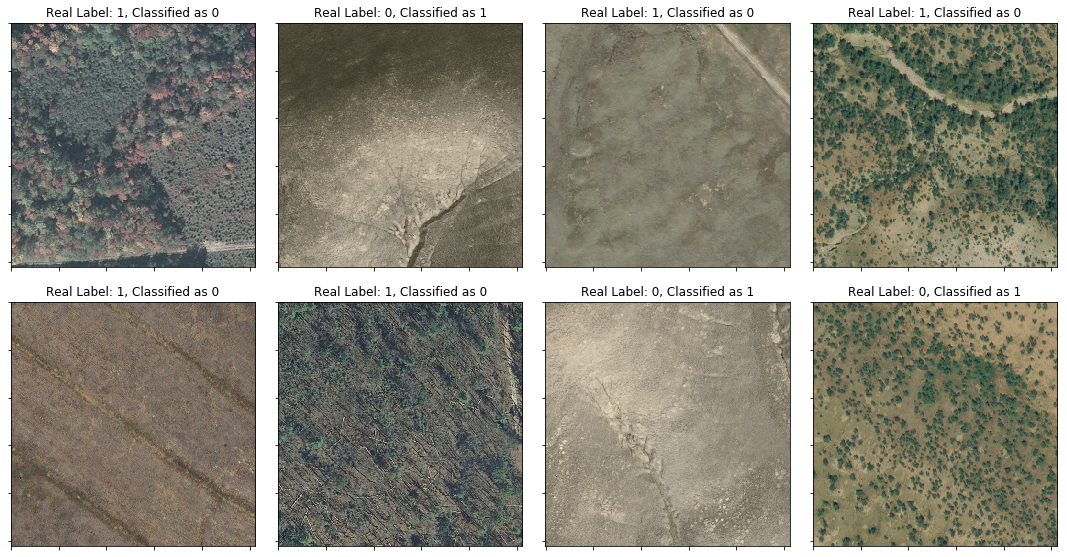
\includegraphics[width=1\textwidth]{Figures/results/class_dataset03m_res03_wrong.png}
	\caption{\textbf{Examples of wrongly classified images at base resolution of the 0.3m dataset.}}
	\label{fig:dataset03m_res03_wrong}
\end{figure}

A similar analysis can be done for the last resolution, 4.8m, of the 0.3m dataset, which is shown in Figs.~\ref{fig:dataset03m_res48_correct} and \ref{fig:dataset03m_res48_wrong}. The first set of images (Fig.~\ref{fig:dataset03m_res48_correct}) indicates that the model detects human impact when it is still evident, even with the low resolution. However, the second set of images (Fig.~\ref{fig:dataset03m_res48_wrong}) implies that it commits errors when the evidence associated to man-made structures is lost with the downgrade process. Similarly, it might classify as man-made structures patterns that are indeed natural.

\begin{figure}[H]
	\centering
	\captionsetup{width=1\linewidth}
	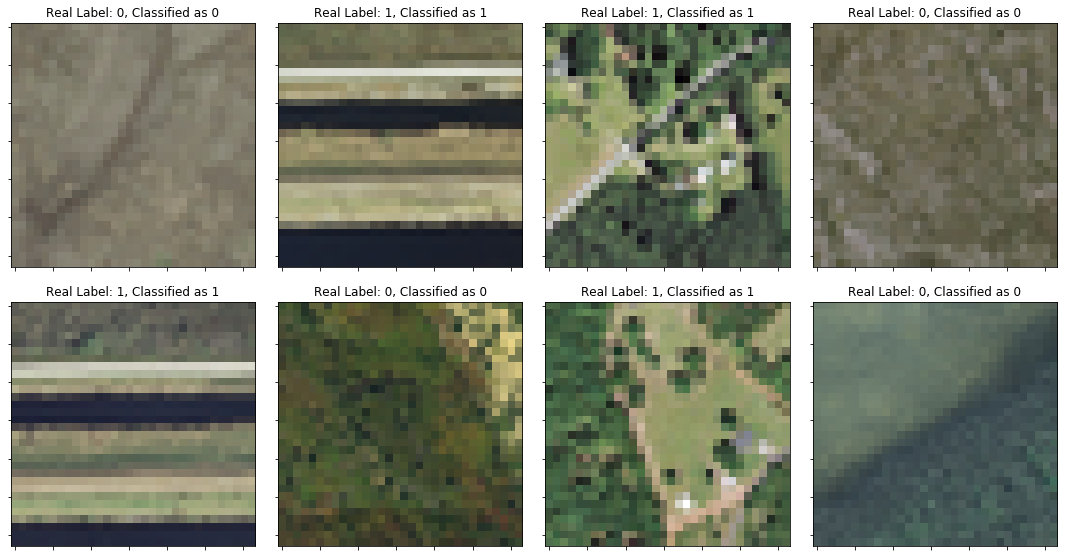
\includegraphics[width=1\textwidth]{Figures/results/class_dataset03m_res48_correct.png}
	\caption{\textbf{Examples of correctly classified images at last resolution, 4.8m, of 0.3m dataset.}}
	\label{fig:dataset03m_res48_correct}
\end{figure}

\begin{figure}[H]
	\centering
	\captionsetup{width=1\linewidth}
	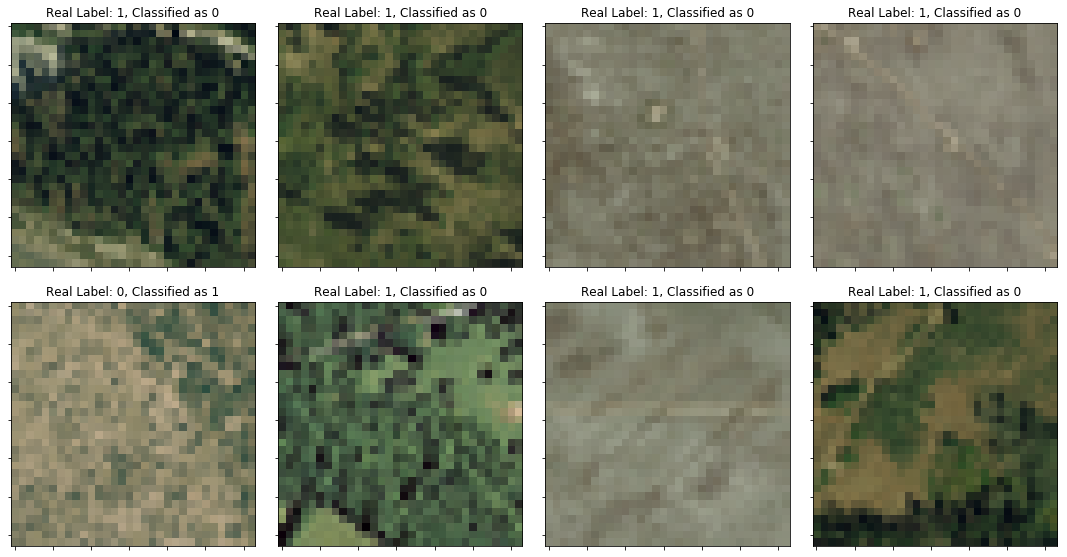
\includegraphics[width=1\textwidth]{Figures/results/class_dataset03m_res48_wrong.png}
	\caption{\textbf{Examples of wrongly classified images at the last resolution, 4.8m, of 0.3m dataset.}}
	\label{fig:dataset03m_res48_wrong}
\end{figure}

These observations are highlighted in Fig.~\ref{fig:dataset03m_res03_res48_comp}, in which we show images that are correctly classified at 0.3m resolution (top row) but wrongly classified at 4.8m. The first and third pair of images demonstrate that, when the human impact is subtle, the model missed it in the downgraded resolution. Conversely, non human activity can also be misclassified at lower resolutions (second and fourth images).

\begin{figure}[H]
	\centering
	\captionsetup{width=1\linewidth}
	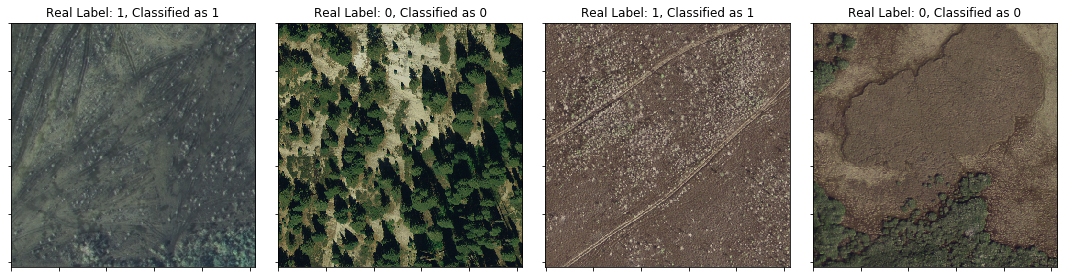
\includegraphics[width=1\textwidth]{Figures/results/class_dataset03m_res03_comp_correct.png}
	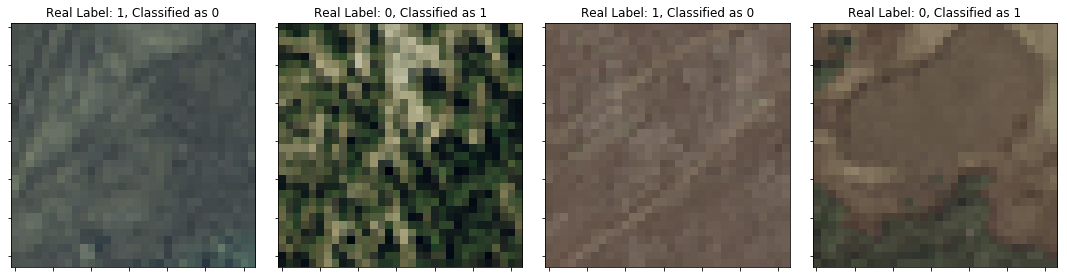
\includegraphics[width=1\textwidth]{Figures/results/class_dataset03m_res48_comp_wrong.png}
	\caption{\textbf{Correctly and wrongly classified images at different resolutions.} Here the first row displays images in their base resolution, 0.3m. These images were correctly classified by the model. The same images at a resolution of 4.8m (second row) were wrongly classified by the model.}
	\label{fig:dataset03m_res03_res48_comp}
\end{figure}

Finally, we investigate how the model behaves with images where human impact is very minimal. For this purpose, we consider the images with the intermediate label (label 1 in Chapter \ref{Chapter2}, Figure \ref{fig:imstats}). The model has never been faced with these images, so this can give a good perception of whether the model has been able to learn relevant features of human impact. Figure \ref{fig:dataset03m_res03_l1} shows several images with the label, that the model predicted, in the title. Even if man-made structures in these pictures are small, the model is able to detect straight lines and shapes as human activity. 

\begin{figure}[H]
	\centering
	\captionsetup{width=1\linewidth}
	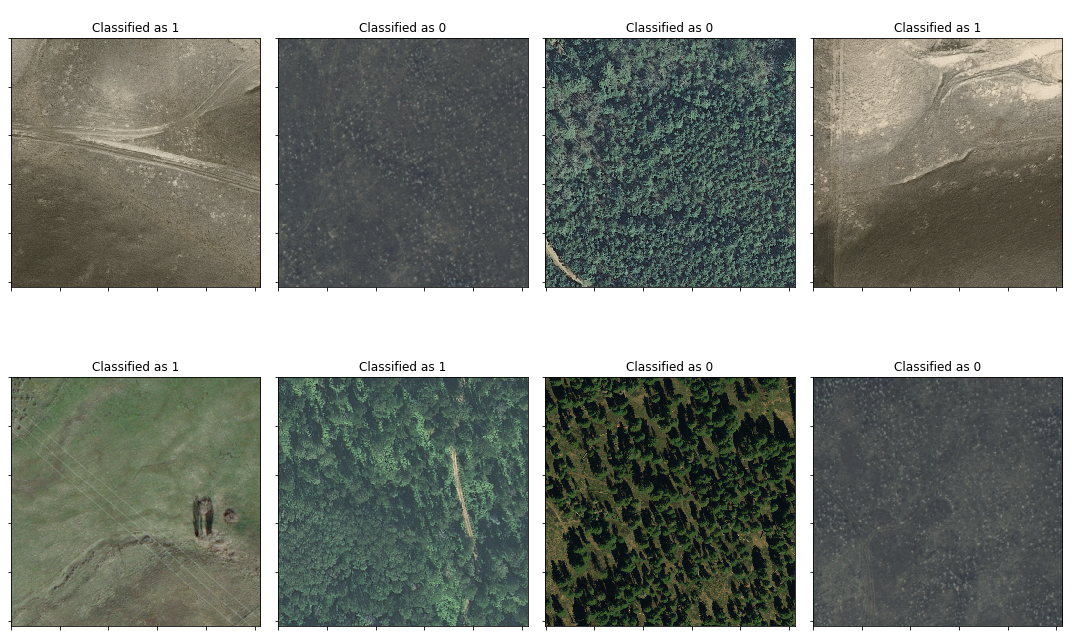
\includegraphics[width=1\textwidth]{Figures/results/class_dataset03m_res03_l1.png}
	\caption{\textbf{Examples of predictions made for images with subtle human impact}. These images were not used when training the model.}
	\label{fig:dataset03m_res03_l1}
\end{figure}

\section{Cost estimation}

We discuss the financial cost associated to building and launching a satellite, and to renting infrastructure for performing the entire image processing pipeline. We further study the cost as a function of pixel resolution. However, our estimates are very rough approximations because many factors are involved and large variations occur between them. To give an example, choosing one material over the other might change the cost of manufacturing and launching a satellite by one order of magnitude. It is also completely different to have a satellite for 3 years in space, or to target a lifespan of 20 years. 

Having this in mind, we follow laws from physics to estimate the dependency of the satellite cost on resolution. First, the cost of launching a satellite into the orbit scales linearly with its mass \parencite{rocket_equation}, which is given by the amount of fuel needed. Second, the mass of the satellite scales quadratic with resolution so that overall we obtain a cubic dependency for launching a satellite into space. The latter increase in cost is associated with the optical instruments used. As a reference for the satellite cost we use a Skysat satellite from Planet \parencite{skysat_planet} that has a resolution of about 1m and a value of $\$30$ million. This amount was provided to us by Satellogic and includes construction, launch and maintenance during the satellite's lifespan.

Our final goal is to give an estimation of the expenditure to monitor once the entire surface of the earth (about 149 million km$^2$). To this end, we multiply the satellite cost by the ratio: time needed to scan the earth over the satellite's lifespan. Further, a satellite can map 1 million km$^2$ at 1m resolution in 4.2 days \parencite{satellogic_youtube}. We hence can calculate the satellite cost per km$^2$. Assuming a lifespane of 10 years we have $area = 10^6 \times \frac{10\cdot365}{4.2}~km^2$ so we obtain $cost~satellite~per~km^2 = cost~satellite/area \approx 0.035~\$/km^2$.

\begin{table}[h!]
	\begin{tabular}{l | l | l | l | l}
		description & cost & unit & cost (\$/km$^2$) & cost (\$/pixel) \\
		\hline
		process raw data & & & 0.004 & $4 \times 10^{-9}$ \\
		hot storage  & $72\times 10^{-6}$ & \$/(km$^2$/month) & 0.000864 & $8.64\times10^{-10}$ \\
		cold storage  & $36\times 10^{-6}$ & \$/(km$^2$/month) & 0.000432 & $4.32\times10^{-10}$ \\
		archive storage  & $9\times 10^{-6}$ & \$/(km$^2$/month) & 0.000108 & $1.08\times10^{-10}$ \\
		download data & 8 & \$/Gb & 0.021 & $2.1  \times 10^{-8}$\\
		serving to final client & 0.09 & \$/Gb & 0.000236 & $4.7232 \times 10^{-10}$\\
		prediction (AWS) & 0.05 \& $\sim$6 & \$/h \& s/km$^2$ & 0.00145 & $1.45 \times 10^{-9}$\\
	\end{tabular}
	\captionsetup{width=1\linewidth}
	\caption{\textbf{Costs for image data processing.} All costs except the prediction are provided by Satellogic.}
	\label{table:data_costs}	
\end{table}

Another cost intensive block when capturing satellite imagery involves image data processing for which the cost scales quadratic with resolution. For example, an operation that costs 100\$/km$2$ at 1m resolution will cost only 1\$/km$^2$ at 10m resolution. The data processing step consists of multiple parts: transformation of raw data into image pixels, storing data in a hot, cold, and archive storage, downloading data from the satellite, serving it to the final client, and in our case predicting human impact. These costs are summarized for 1m resolution in table \ref{table:data_costs}. Note that we used the conversion factor 0.002624 for an image to convert from Gigabytes to km$^2$ (2$\times$ compressed) and we assume 12 months of data storage. 

The prediction step is estimated by loading 4 images that each have an area of about $500\times500m^2$, calculating the ResNet activations of the final layer, and predicting the class using the models trained in chapter~\ref{Chapter4} in an ensemble fashion. This part amounts to a processing time of about 6s for an area of 1km$^2$, which can be converted into costs per km$^2$ assuming 0.05\$/h of AWS EC2 compute~\parencite{aws}.

To finally obtain the dependence of the resolution on the total financial cost we sum the data cost per km$^2$ and the satellite cost per km$^2$ at 1m resolution, and convert to cost per pixel ($\times 10^{-6}$). We then multiply with the number of pixels necessary to cover the entire surface of the earth. Here the satellite cost per km$^2$ is a cubic function and the earth surface in pixel is a quadratic function in resolution. The result is shown in Fig.~\ref{fig:costs}. We obtain a cost of about \$15 million dollars at 1m resolution with a very steep slope towards better resolutions. At 0.3m resolution the cost is two orders of magnitude higher than at 1m while for worse resolutions the cost decreases by two orders of magninute when the resolution is about 10m. We conclude that for worse resolutions the data processing cost is the dominating cost whereas for very good resolutions the satellite cost dominates.

\begin{figure}[h!]
	\centering
	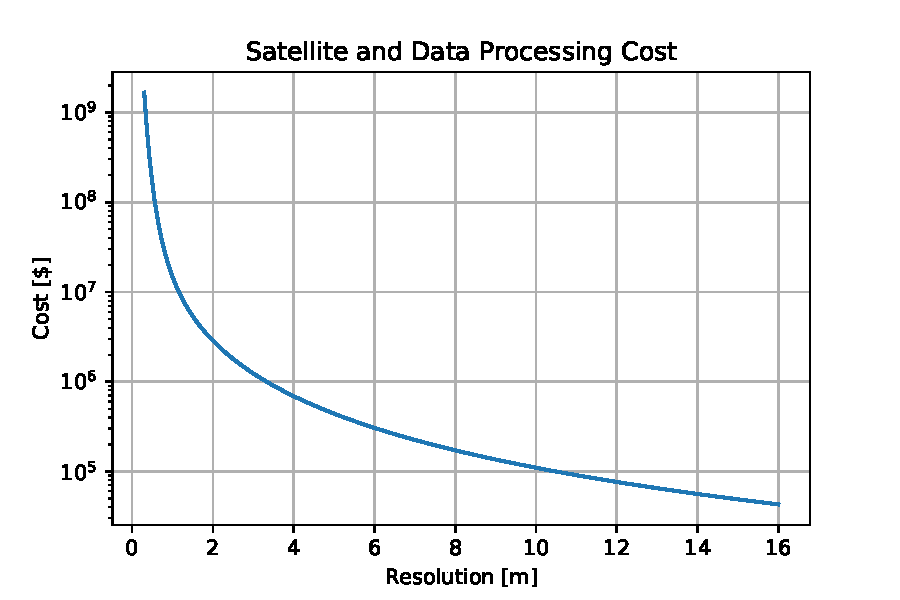
\includegraphics[width=0.75\textwidth]{Figures/costs.pdf}
	\captionsetup{width=1\linewidth}
	\caption{\textbf{Satellite and data processing cost.} The total financial cost to capture images with a satellite and process the data as function of resolution.}
	\label{fig:costs}
\end{figure}


